\section{Тестирование работоспособности программного средства}

\subsection{Тестирование модуля построения маршрута}

Цель -- убедиться, что робот может перемещаться из точки A в точку B по прямой
линии без препятствий.
Метод -- симуляторе Webots была создана простая среда без
объектов, и роботу была задана задача достичь целевой точки.
Результат -- робот успешно достиг целевой точки, продемонстрировав корректную
работу датчиков и базового алгоритма движения.

\FloatBarrier
\begin{figure}[h]
\centering
	\fbox{
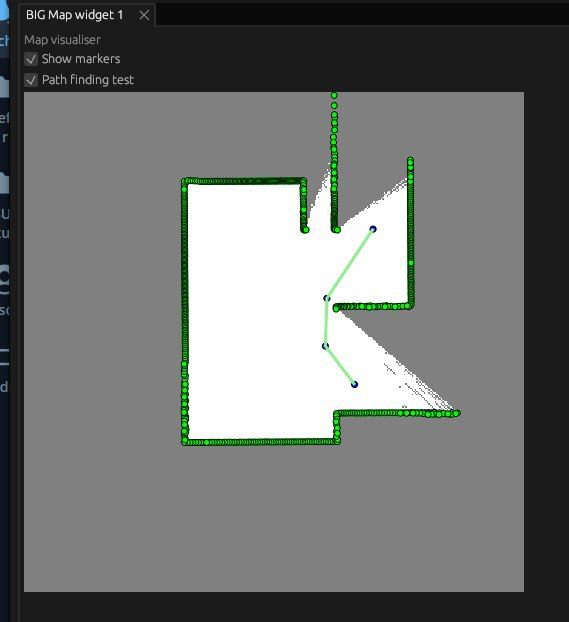
\includegraphics[width=14cm]{global_planner}
}
\caption{Тестирование построение маршрута}
\end{figure}
\FloatBarrier

\subsection{Тестирование модуля наложения снимков лидара}

Цель -- проверить, как алгоритм строит маршрут, обходя неподвижные объекты.
Метод -- в среде были размещены стены и коробки, и роботу была задана задача их
обойти.

\FloatBarrier
\begin{figure}[h]
\centering
	\fbox{
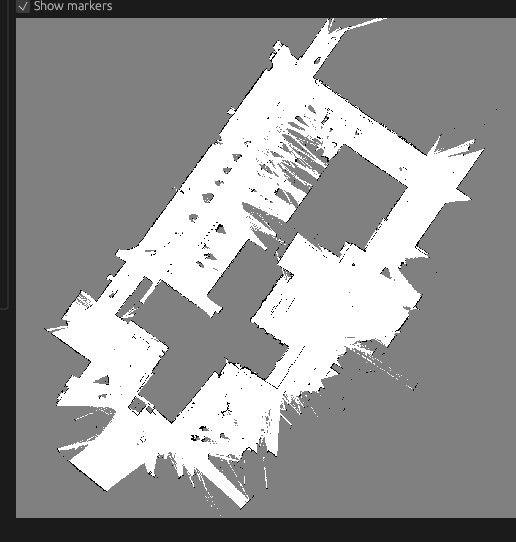
\includegraphics[width=14cm]{bsuir_dorm2_example}
}
\caption{Карта местности вокруг Общежития \No{2} БГУИР}
\end{figure}
\FloatBarrier

Результат -- алгоритм точно обнаружил препятствия и спланировал
безопасный путь, избегая столкновений.

\subsection{Тестирование модуля UKF}

Во время тестирования модуль показал исправную работу.

\FloatBarrier
\begin{figure}[h]
\centering
	\fbox{
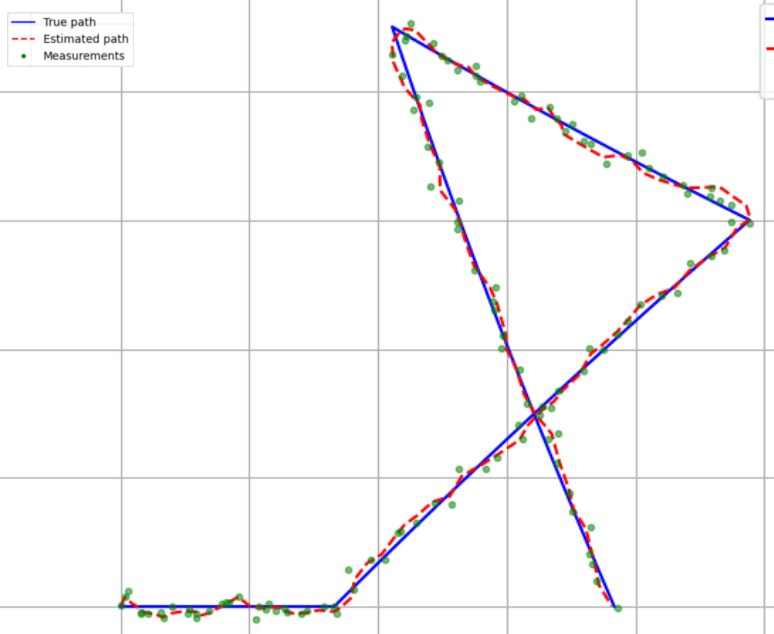
\includegraphics[width=14cm]{ukf_testing}
}
\caption{Тестирование UKF}
\end{figure}
\FloatBarrier

\subsection{Интеграционное тестирование в симуляции}


Цель -- проверить работу алгоритма в запутанных пространствах.
Метод -- была создана карта с множеством поворотов и тупиков.
Результат -- алгоритм нашел оптимальный путь и избежал зацикливания, что
подтверждает его эффективность в сложных условиях.

\FloatBarrier
\begin{figure}[h]
\centering
	\fbox{
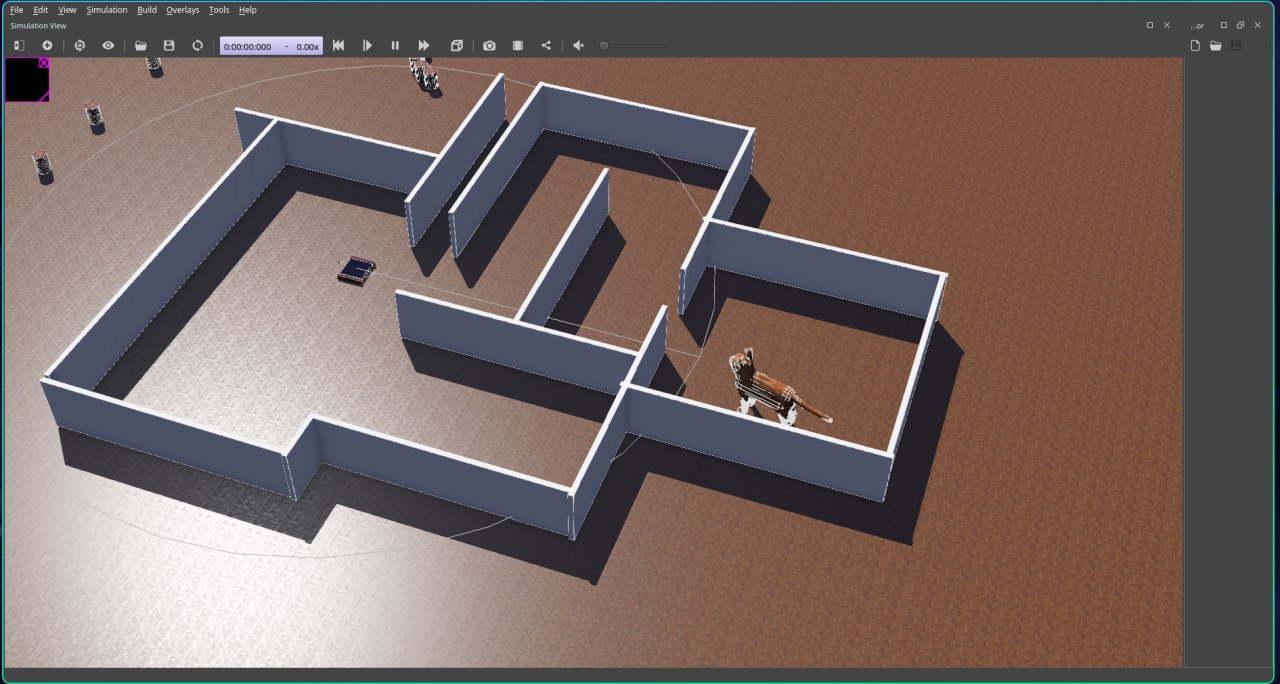
\includegraphics[width=8cm]{webots_screenshot}
}
\caption{Среда симуляции Webots}
\end{figure}
\FloatBarrier


Все проведенные тесты были успешно пройдены, что подтверждает высокую
эффективность, надежность и адаптивность разработанного алгоритма построения
карты и нахождения пути. Результаты тестирования позволяют рекомендовать данный
алгоритм для использования в реальных условиях.

% \subsection{Интеграционное тестирование на роботе}
% \todo{Робот катается IRL}

